%%%%%%%%%%%%%%%%%%%%%%%%%%%%%%%%%%%%%%%%%%%%%%%%%%%%%%%%%%%%%%%%%%%
%                                                                 %
%                            CHAPTER SIX                          %
%                                                                 %
%%%%%%%%%%%%%%%%%%%%%%%%%%%%%%%%%%%%%%%%%%%%%%%%%%%%%%%%%%%%%%%%%%%

\chapter{MBVL CLASSIFICATION}

\section{Versioning Graph}

The experiment undergoes two phases of comparison in this procedure.
The first phase compares the initial species content with the classifications by a particular algorithm/taxonomy combination.
Since the classification results from a population selected according to the initial species list, these two datasets share a common provenance.
However, the list cannot be used in place of the classifier results because not only does it have only 21 entries, but also it does not have a clear correspondence with the DNA chains sent to the classifier.
As a result, these two sets are no versions of each other, and versioning results will have weak implications.
A labeling of the initial input data, alternatively would be considered a version of the results, but that data product is not available.

Each taxonomy and classifier combination outputs a taxonomic classification for each entry from the same source.
Shared input data indicates the results share common provenance.
The classifications also share the same workflow step because their results have similar formats, reporting a specific taxonomic name for each entry.
Since classifications occur over the same set of entries, their identifiers can be used to match outputs together for comparison.
However, the classifiers do not identify entries to the same specificity.
If it determines that the confidence at a particular rank is too low, it marks that level as ambiguous and computes no further ranks.
As a result, versioning can determine additions and invalidations based on whether a classifier can ascertain more or less of an entry's taxonomic name.
This method of mapping the versions together allows the results to give insight into the accuracy of different algorithm and taxonomy combinations.

\begin{figure}
	\centering
	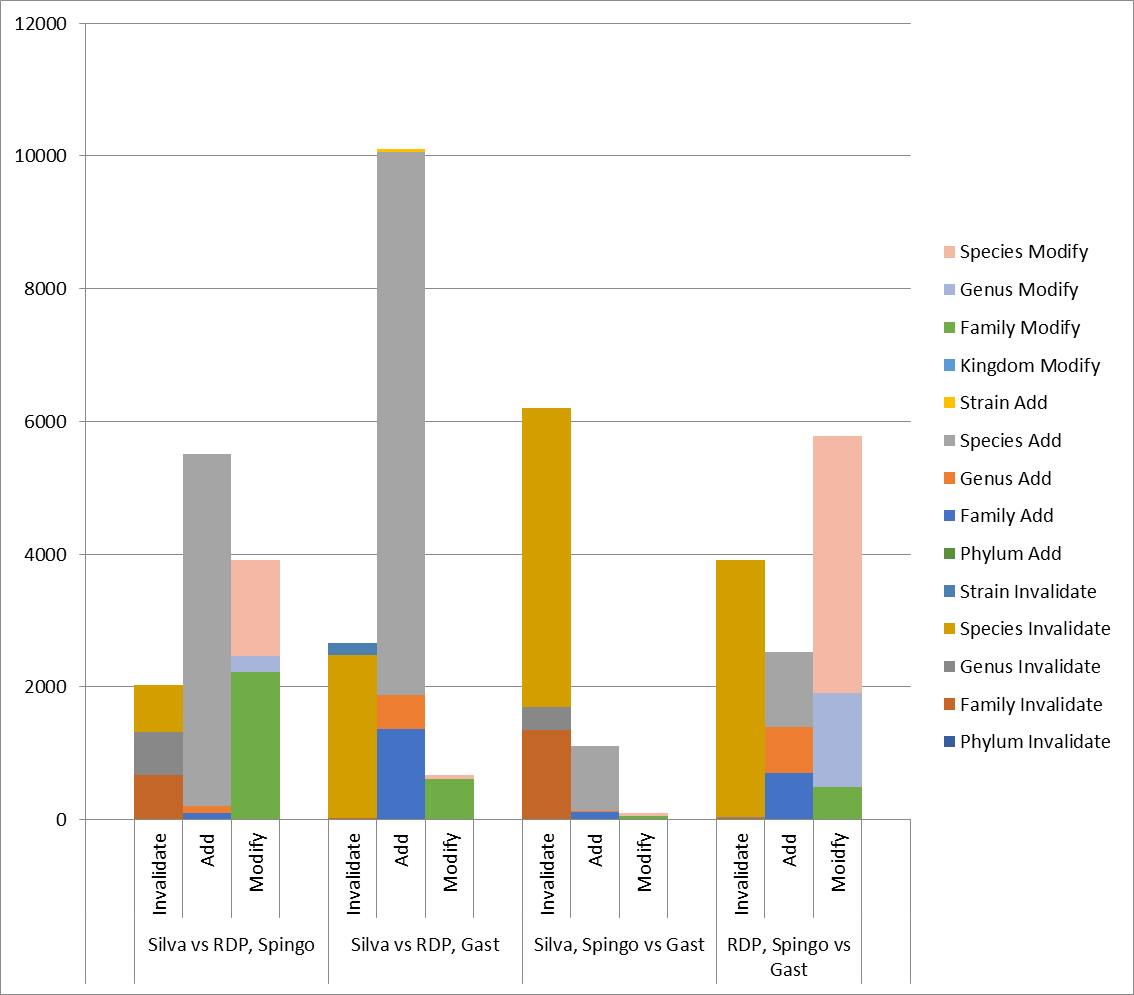
\includegraphics[scale=0.80]{figures/mbvl_chart.png}
	\caption{Compiled counts of adds, invalidates, and modifies grouped by taxonomic rank across algorithm and taxonomy combinations.}
	\label{mbvl_chart}
\end{figure}